\documentclass[11pt,spanish]{article} % Idioma
\usepackage{babel}
\usepackage[T1]{fontenc}
\usepackage{textcomp}
\usepackage[utf8]{inputenc} % Puede depender del instrucción, sistema o editor
\usepackage{wrapfig} % Imagenes
% \graphicspath{ {./imagenes/} }

\usepackage[left=2.75cm,top=2.5cm,right=2cm,bottom=2.5cm]{geometry} % Márgenes
%\usepackage{pstricks} % Gráficas, movilidad, árboles y otros

\usepackage{amssymb, amsmath} % Símbolos matemáticos
\usepackage{amsthm} % Teoremas, lemas, pruebas...
\usepackage{cancel} % Cancelar expresiones
\usepackage{multirow} % Tablas
\usepackage{multicol}

\usepackage{graphicx} % Inserción de imágenes
\usepackage{xcolor} % Colores
\usepackage{color}
\definecolor{gray97}{gray}{.97}
\definecolor{gray75}{gray}{.75}
\definecolor{gray45}{gray}{.45}

\usepackage[hidelinks]{hyperref}  % Enlaces
\usepackage{multirow} % Tablas

\usepackage{listings} % Escribir código en diferentes lenguajes de programación
\usepackage{longtable} % para tablas largas
\lstset{ frame=Ltb,
framerule=0pt,
aboveskip=0.5cm,
framextopmargin=3pt,
framexbottommargin=3pt,
framexleftmargin=0.4cm,
framesep=0pt,
rulesep=.4pt,
backgroundcolor=\color{gray97},
rulesepcolor=\color{black},
%
stringstyle=\ttfamily,
showstringspaces = false,
basicstyle=\small\ttfamily,
commentstyle=\color{gray45},
keywordstyle=\bfseries,
%
numbers=left,
numbersep=15pt,
numberstyle=\tiny,
numberfirstline = false,
breaklines=true,
}



\title{Memoria de algor\'itmica}
\author{Rubén Morales Pérez
		\and Francisco Javier Morales Piqueras
		\and Bruno Santindrian Manzanedo
		\and Ignacio de Loyola Barragan Lozano
		\and Francisco Leopoldo Gallego Salido}
\date{\today}


% % % % % % % % % % % % % % % % % % % % % % % % % % % % % % % % %
%					 Inicio del documento
% % % % % % % % % % % % % % % % % % % % % % % % % % % % % % % % %
\begin{document}
\maketitle
\tableofcontents % Generando el indice
\newpage
\setlength\parindent{0pt} % Quitamos la sangría

%%%%%%%%%%%%%%%%%%%%%%%%%%%%%%%%%%%%%%%%%%%%%%%%%%%%%%%%%%%%%%%%%%%%%%%%%%%%%%%%%%


\section{Explicaci\'on del m\'etodo utilizado}
Para la obtenci\'on de los datos deseados hemos realizado un script de bash que genera las tablas de datos y las gráficas con su correspondiente ajuste.
\begin{lstlisting}[language=bash]
#!/bin/bash

if [ $# -ne 1 ]
then
    echo "Uso: $0 <nombre>"
    exit 1
fi

# HEAPSORT
g++ -std=c++11 ../src/heapsort.cpp
nelementos=200
echo "" > datos.dat
while [ $nelementos -lt 10000 ]; do
    ./a.out $nelementos >> datos.dat
    let nelementos=nelementos+100
done

gnuplot ./gnuplot/heapsort.gp # Salida: "fichero.jpeg"

mkdir ../Graficas/Heapsort 2> /dev/null
mkdir ../Graficas/Heapsort/Datos 2> /dev/null
mv fichero.jpeg ../Graficas/Heapsort/heapsortO0_$1.jpeg
mv datos.dat ../Graficas/Heapsort/Datos/heapsortO0_$1.dat
echo "Heapsort completado"


# MERGESORT
g++ -std=c++11 ../src/mergesort.cpp
nelementos=200
echo "" > datos.dat
while [ $nelementos -lt 10000 ]; do
    ./a.out $nelementos >> datos.dat
    let nelementos=nelementos+100
done

gnuplot ./gnuplot/mergesort.gp # Salida: "fichero.jpeg"

mkdir ../Graficas/Mergesort 2> /dev/null
mkdir ../Graficas/Mergesort/Datos 2> /dev/null
mv fichero.jpeg ../Graficas/Mergesort/mergesortO0_$1.jpeg
mv datos.dat ../Graficas/Mergesort/Datos/mergesortO0_$1.dat
echo "Mergesort completado"


# INSERCION
g++ -std=c++11 ../src/insercion.cpp
nelementos=200
echo "" > datos.dat
while [ $nelementos -lt 10000 ]; do
    ./a.out $nelementos >> datos.dat
    let nelementos=nelementos+100
done

gnuplot ./gnuplot/insercion.gp # Salida: "fichero.jpeg"

mkdir ../Graficas/Insercion 2> /dev/null
mkdir ../Graficas/Insercion/Datos 2> /dev/null
mv fichero.jpeg ../Graficas/Insercion/insercionO0_$1.jpeg
mv datos.dat ../Graficas/Insercion/Datos/insercionO0_$1.dat
echo "Insercion completado"


# SELECCION
g++ -std=c++11 ../src/seleccion.cpp
nelementos=200
echo "" > datos.dat
while [ $nelementos -lt 10000 ]; do
    ./a.out $nelementos >> datos.dat
    let nelementos=nelementos+100
done

gnuplot ./gnuplot/insercion.gp # Salida: "fichero.jpeg"

mkdir ../Graficas/Seleccion 2> /dev/null
mkdir ../Graficas/Seleccion/Datos 2> /dev/null
mv fichero.jpeg ../Graficas/Seleccion/seleccionO0_$1.jpeg
mv datos.dat ../Graficas/Seleccion/Datos/seleccionO0_$1.dat
echo "Seleccion completado"


# QUICKSORT
g++ -std=c++11 ../src/quicksort.cpp
nelementos=200
echo "" > datos.dat
while [ $nelementos -lt 10000 ]; do
    ./a.out $nelementos >> datos.dat
    let nelementos=nelementos+100
done

gnuplot ./gnuplot/quicksort.gp # Salida: "fichero.jpeg"

mkdir ../Graficas/Quicksort 2> /dev/null
mkdir ../Graficas/Quicksort/Datos 2> /dev/null
mv fichero.jpeg ../Graficas/Quicksort/quicksortO0_$1.jpeg
mv datos.dat ../Graficas/Quicksort/Datos/quicksortO0_$1.dat
echo "Quicksort completado"


# BURBUJA
g++ -std=c++11 ../src/burbuja.cpp
nelementos=200
echo "" > datos.dat
while [ $nelementos -lt 10000 ]; do
    ./a.out $nelementos >> datos.dat
    let nelementos=nelementos+100
done

gnuplot ./gnuplot/burbuja.gp # Salida: "fichero.jpeg"

mkdir ../Graficas/Burbuja 2> /dev/null
mkdir ../Graficas/Burbuja/Datos 2> /dev/null
mv fichero.jpeg ../Graficas/Burbuja/burbujaO0_$1.jpeg
mv datos.dat ../Graficas/Burbuja/Datos/burbujaO0_$1.dat
echo "Burbuja completado"


# FIBONACCI
g++ -std=c++11 ../src/fibonacci.cpp
nelementos=1
echo "" > datos.dat
while [ $nelementos -lt 50 ]; do
    ./a.out $nelementos >> datos.dat
    let nelementos=nelementos+2
done

gnuplot ./gnuplot/fibonacci.gp # Salida: "fichero.jpeg"

mkdir ../Graficas/Fibonacci 2> /dev/null
mkdir ../Graficas/Fibonacci/Datos 2> /dev/null
mv fichero.jpeg ../Graficas/Fibonacci/fibonacciO0_$1.jpeg
mv datos.dat ../Graficas/Fibonacci/Datos/fibonacciO0_$1.dat
echo "Fibonacci completado"


# HANOI
g++ -std=c++11 ../src/hanoi.cpp
nelementos=3
echo "" > datos.dat
while [ $nelementos -lt 30 ]; do
    ./a.out $nelementos >> datos.dat
    let nelementos=nelementos+1
done

gnuplot ./gnuplot/hanoi.gp # Salida: "fichero.jpeg"

mkdir ../Graficas/Hanoi 2> /dev/null
mkdir ../Graficas/Hanoi/Datos 2> /dev/null
mv fichero.jpeg ../Graficas/Hanoi/hanoiO0_$1.jpeg
mv datos.dat ../Graficas/Hanoi/Datos/hanoiO0_$1.dat
echo "Hanoi completado"


# FLOYD
g++ -std=c++11 ../src/floyd.cpp
nelementos=200
echo "" > datos.dat
while [ $nelementos -lt 1000 ]; do
    ./a.out $nelementos >> datos.dat
    let nelementos=nelementos+10
done

gnuplot ./gnuplot/floyd.gp # Salida: "fichero.jpeg"

mkdir ../Graficas/Floyd 2> /dev/null
mkdir ../Graficas/Floyd/Datos 2> /dev/null
mv fichero.jpeg ../Graficas/Floyd/floydO0_$1.jpeg
mv datos.dat ../Graficas/Floyd/Datos/floydO0_$1.dat
echo "Floyd completado"

rm a.out
rm fit.log
\end{lstlisting}

Para la obtención de las gráficas de forma directa utilizamos script de gnuplot que tienen la forma siguiente, en este caso adjuntamos "burbuja.gp".

\begin{lstlisting}[language=gnuplot]
set terminal jpeg
set output "fichero.jpeg"

set title "Eficiencia burbuja"
set xlabel "Tamano del vector"
set ylabel "Tiempo (s)"
set fit quiet
f(x) = a*x*x+b*x+c
fit f(x) "datos.dat" via a, b, c
plot "datos.dat", f(x)
\end{lstlisting}

Los diferentes ajustes se han conseguido así:

\begin{lstlisting}[language=gnuplot]
f(x) = a*x*x*x+b*x*x+c*x+d
g(x) = a*x*x+b*x+c
h(x) = a*x*(log(x)/log(2))
i(x) = a*(((1+sqrt(5))/2)**x)
\end{lstlisting}

\subsection{Comparativa entre diferentes ordenadores}
Para conseguir las gráficas con  todos los datos hemos usado otro script de bash.

\begin{lstlisting}[language=gnuplot]
\#!/bin/bash
for DIR in `ls Graficas/`; do
  if [ $DIR != Ajustes ] && [ -d Graficas/$DIR ]
    then
    archivo="temporal.gp"

    echo "set terminal jpeg" > \$archivo
    echo "set output \"fichero.jpeg\"" >> $archivo
    echo "set title \"Eficiencia $DIR\"" >> $archivo
    echo "set xlabel \"Tamano del vector\"" >> $archivo
    echo "set ylabel \"Tiempo (s)\"" >> $archivo
    echo "set fit quiet" >> $archivo
    echo "unset key" >> $archivo

    num=0
    dir="Graficas/$DIR/Datos"

    for FILE in `ls $dir`; do
      if [ $DIR == Burbuja ] || [ $DIR == Insercion ] || [ $DIR == Seleccion ]
        then
        echo "f$num(x) = a*x*x+b*x+c" >> $archivo
        echo "fit f$num(x) \"$dir/$FILE\" via a, b, c" >> $archivo
      elif [ $DIR == Mergesort ] || [ $DIR == Quicksort ] || [ $DIR == Heapsort ]
        then
        echo "f$num(x) = a*x*(log(x)/log(2))" >> $archivo
        echo "fit f$num(x) \"$dir/$FILE\" via a" >> $archivo
      elif [ $DIR == Fibonacci ]
        then
        echo "f$num(x) = a*(((1+sqrt(5))/2)**x)" >> $archivo
        echo "fit f$num(x) \"$dir/$FILE\" via a" >> $archivo
      elif [ $DIR == Floyd ]
        then
        echo "f$num(x) = a*x*x*x+b*x*x+c*x+d" >> $archivo
        echo "fit f$num(x) \"$dir/$FILE\" via a, b, c, d" >> $archivo
      elif [ $DIR == Hanoi ]
        then
        echo "f$num(x) = a*(2**x)" >> $archivo
        echo "fit f$num(x) \"$dir/$FILE\" via a" >> $archivo
      fi

      let num=num+1
    done

    num=0
    printf "plot" >> $archivo

    for FILE in `ls $dir`; do
      if [ $num == 0 ]
        then
        printf  " \"$dir/$FILE\", f$num(x)" >> $archivo
      else printf ", \"$dir/$FILE\", f$num(x)" >> $archivo
      fi

      let num=num+1
    done

    gnuplot ./temporal.gp
    mv fichero.jpeg ./Graficas/$DIR/total_$DIR.jpeg
  fi
done

rm temporal.gp
rm fit.log
\end{lstlisting}

\newpage
%%%%%%%%%%%%%%%%%%%%%%%%%%%%%%%%%%%%%%%%%%%%%%%%%%%%%%%%%%%%%

\section{C\'alculo de la eficiencia emp\'irica}
%\hspace*{1cm}\textbf{Ejercicio 1.}

\subsection{Tabla con los algor\'itmos cuadr\'aticos}
	\begin{center}
	\begin{longtable}{|l||l|l|l|}
	\hline
	\multicolumn{1}{|c||}{N} & \multicolumn{1}{c|}{BURBUJA} & \multicolumn{1}{c|}{INSERCIÓN} & \multicolumn{1}{c|}{SELECCIÓN} \\ \hline
200                     & 0.000144071                  & 4.7705e-05                     & 8.5147e-05                     \\ \hline
300                     & 0.000231713                  & 0.000115954                    & 0.000178518                    \\ \hline
400                     & 0.000426816                  & 0.000245951                    & 0.000301316                    \\ \hline
500                     & 0.000702491                  & 0.000374198                    & 0.000470279                    \\ \hline
600                     & 0.00105612                   & 0.000513312                    & 0.000632222                    \\ \hline
700                     & 0.00140341                   & 0.000550801                    & 0.000675113                    \\ \hline
800                     & 0.00183138                   & 0.000752914                    & 0.000886985                    \\ \hline
900                     & 0.00222473                   & 0.000898051                    & 0.0011041                      \\ \hline
1000                    & 0.0027604                    & 0.00111676                     & 0.00134688                     \\ \hline
1100                    & 0.00354976                   & 0.00134434                     & 0.00158277                     \\ \hline
1200                    & 0.00406315                   & 0.00160836                     & 0.00190872                     \\ \hline
1300                    & 0.00471413                   & 0.00196183                     & 0.00218885                     \\ \hline
1400                    & 0.00569382                   & 0.00219148                     & 0.00250872                     \\ \hline
1500                    & 0.00634717                   & 0.00249123                     & 0.00291645                     \\ \hline
1600                    & 0.00741644                   & 0.00289297                     & 0.00336508                     \\ \hline
1700                    & 0.00838426                   & 0.00324374                     & 0.00371176                     \\ \hline
1800                    & 0.00925945                   & 0.00356608                     & 0.0041016                      \\ \hline
1900                    & 0.0103737                    & 0.00403539                     & 0.00456578                     \\ \hline
2000                    & 0.0113986                    & 0.00429669                     & 0.00522582                     \\ \hline
2100                    & 0.0125963                    & 0.00479624                     & 0.00552838                     \\ \hline
2200                    & 0.0137679                    & 0.00529551                     & 0.00619605                     \\ \hline
2300                    & 0.0150761                    & 0.00579104                     & 0.00667429                     \\ \hline
2400                    & 0.01632                      & 0.00625809                     & 0.00726558                     \\ \hline
2500                    & 0.0178993                    & 0.006999                       & 0.00789763                     \\ \hline
2600                    & 0.019347                     & 0.00733744                     & 0.00845852                     \\ \hline
2700                    & 0.0215196                    & 0.00795048                     & 0.00918807                     \\ \hline
2800                    & 0.0229786                    & 0.00854829                     & 0.00982301                     \\ \hline
2900                    & 0.0241723                    & 0.00942415                     & 0.0105492                      \\ \hline
3000                    & 0.0256532                    & 0.0100209                      & 0.011249                       \\ \hline
3100                    & 0.0275161                    & 0.010457                       & 0.0120472                      \\ \hline
3200                    & 0.0295651                    & 0.011138                       & 0.012849                       \\ \hline
3300                    & 0.0311401                    & 0.0117862                      & 0.0135953                      \\ \hline
3400                    & 0.0332632                    & 0.0125172                      & 0.0144005                      \\ \hline
3500                    & 0.0352209                    & 0.0132863                      & 0.0151668                      \\ \hline
3600                    & 0.0372677                    & 0.0140734                      & 0.0161134                      \\ \hline
3700                    & 0.039705                     & 0.0148475                      & 0.0170161                      \\ \hline
3800                    & 0.0417078                    & 0.0156604                      & 0.0179772                      \\ \hline
3900                    & 0.0435252                    & 0.0197043                      & 0.0188737                      \\ \hline
4000                    & 0.0458737                    & 0.0181161                      & 0.0199172                      \\ \hline
4100                    & 0.0478526                    & 0.0181901                      & 0.0207891                      \\ \hline
4200                    & 0.0507376                    & 0.0190718                      & 0.0218186                      \\ \hline
4300                    & 0.053108                     & 0.0202904                      & 0.0229509                      \\ \hline
4400                    & 0.0558002                    & 0.0210508                      & 0.0239336                      \\ \hline
4500                    & 0.0582709                    & 0.0217675                      & 0.0251007                      \\ \hline
4600                    & 0.0602694                    & 0.0229438                      & 0.0262614                      \\ \hline
4700                    & 0.0642321                    & 0.0237263                      & 0.0279806                      \\ \hline
4800                    & 0.0663165                    & 0.0258871                      & 0.0290361                      \\ \hline
4900                    & 0.0686783                    & 0.0262065                      & 0.0296667                      \\ \hline
5000                    & 0.0730717                    & 0.0270327                      & 0.0308016                      \\ \hline
5100                    & 0.0753673                    & 0.0279962                      & 0.0325486                      \\ \hline
5200                    & 0.0780246                    & 0.0290147                      & 0.0335079                      \\ \hline
5300                    & 0.0812102                    & 0.0303489                      & 0.0349218                      \\ \hline
5400                    & 0.0844811                    & 0.0316631                      & 0.0359627                      \\ \hline
5500                    & 0.0875461                    & 0.0326034                      & 0.0371967                      \\ \hline
5600                    & 0.0907043                    & 0.0339502                      & 0.0386688                      \\ \hline
5700                    & 0.0936372                    & 0.0349033                      & 0.0413719                      \\ \hline
5800                    & 0.0974524                    & 0.036554                       & 0.0413017                      \\ \hline
5900                    & 0.101436                     & 0.0373498                      & 0.0427043                      \\ \hline
6000                    & 0.105026                     & 0.0390757                      & 0.0442229                      \\ \hline
6100                    & 0.108229                     & 0.0399669                      & 0.04555                        \\ \hline
6200                    & 0.111798                     & 0.0413162                      & 0.0469907                      \\ \hline
6300                    & 0.115903                     & 0.0425839                      & 0.0487687                      \\ \hline
6400                    & 0.119014                     & 0.0439065                      & 0.0503498                      \\ \hline
6500                    & 0.122901                     & 0.0453498                      & 0.0518471                      \\ \hline
6600                    & 0.126966                     & 0.0467314                      & 0.0544042                      \\ \hline
6700                    & 0.131135                     & 0.0485703                      & 0.0547511                      \\ \hline
6800                    & 0.135234                     & 0.0500184                      & 0.0563988                      \\ \hline
6900                    & 0.138634                     & 0.0521562                      & 0.0582125                      \\ \hline
7000                    & 0.142301                     & 0.0531162                      & 0.0597989                      \\ \hline
7100                    & 0.147276                     & 0.054612                       & 0.0615253                      \\ \hline
7200                    & 0.152644                     & 0.055705                       & 0.0640121                      \\ \hline
7300                    & 0.156869                     & 0.058406                       & 0.0654828                      \\ \hline
7400                    & 0.16054                      & 0.0587351                      & 0.066994                       \\ \hline
7500                    & 0.164664                     & 0.0604273                      & 0.0693313                      \\ \hline
7600                    & 0.169748                     & 0.060933                       & 0.070662                       \\ \hline
7700                    & 0.175759                     & 0.0626671                      & 0.0723676                      \\ \hline
7800                    & 0.178235                     & 0.0641131                      & 0.0740058                      \\ \hline
7900                    & 0.182312                     & 0.0657378                      & 0.0763002                      \\ \hline
8000                    & 0.187312                     & 0.067387                       & 0.0779757                      \\ \hline
8100                    & 0.194597                     & 0.068966                       & 0.0798569                      \\ \hline
8200                    & 0.195945                     & 0.0718069                      & 0.0819951                      \\ \hline
8300                    & 0.199926                     & 0.0721047                      & 0.0841523                      \\ \hline
8400                    & 0.206182                     & 0.074008                       & 0.0858795                      \\ \hline
8500                    & 0.215875                     & 0.0766523                      & 0.088084                       \\ \hline
8600                    & 0.21779                      & 0.0784634                      & 0.0907394                      \\ \hline
8700                    & 0.223402                     & 0.0801562                      & 0.0922715                      \\ \hline
8800                    & 0.227181                     & 0.0847167                      & 0.0953117                      \\ \hline
8900                    & 0.231457                     & 0.0836375                      & 0.0965082                      \\ \hline
9000                    & 0.239053                     & 0.0844739                      & 0.0987032                      \\ \hline
9100                    & 0.246142                     & 0.0863213                      & 0.100973                       \\ \hline
9200                    & 0.249883                     & 0.0894488                      & 0.102804                       \\ \hline
9300                    & 0.252749                     & 0.0911851                      & 0.105066                       \\ \hline
9400                    & 0.257921                     & 0.0923835                      & 0.10754                        \\ \hline
9500                    & 0.262532                     & 0.0946217                      & 0.10974                        \\ \hline
9600                    & 0.267105                     & 0.0967365                      & 0.11298                        \\ \hline
9700                    & 0.273158                     & 0.0994994                      & 0.115105                       \\ \hline
9800                    & 0.278323                     & 0.100605                       & 0.116899                       \\ \hline
9900                    & 0.287314                     & 0.10429                        & 0.119566                       \\ \hline
	\end{longtable}
	\end{center}
	
	
\subsection{Tabla con los algor\'itmos c\'ubicos}
\begin{center}
\begin{longtable}{|c||c|}
\hline
N   & FLOYD     \\ \hline
200 & 0.0442583 \\ \hline
210 & 0.0513714 \\ \hline
220 & 0.0589416 \\ \hline
230 & 0.0668977 \\ \hline
240 & 0.0757302 \\ \hline
250 & 0.0858017 \\ \hline
260 & 0.0960106 \\ \hline
270 & 0.107465  \\ \hline
280 & 0.120661  \\ \hline
290 & 0.134007  \\ \hline
300 & 0.147061  \\ \hline
310 & 0.1623    \\ \hline
320 & 0.178652  \\ \hline
330 & 0.194952  \\ \hline
340 & 0.21375   \\ \hline
350 & 0.233218  \\ \hline
360 & 0.252005  \\ \hline
370 & 0.274844  \\ \hline
380 & 0.296044  \\ \hline
390 & 0.321653  \\ \hline
400 & 0.347014  \\ \hline
410 & 0.371958  \\ \hline
420 & 0.400566  \\ \hline
430 & 0.429389  \\ \hline
440 & 0.462065  \\ \hline
450 & 0.493342  \\ \hline
460 & 0.52677   \\ \hline
470 & 0.560923  \\ \hline
480 & 0.596832  \\ \hline
490 & 0.635627  \\ \hline
500 & 0.673687  \\ \hline
510 & 0.714774  \\ \hline
520 & 0.756145  \\ \hline
530 & 0.802071  \\ \hline
540 & 0.850585  \\ \hline
550 & 0.895673  \\ \hline
560 & 0.945186  \\ \hline
570 & 0.995442  \\ \hline
580 & 1.05703   \\ \hline
590 & 1.10411   \\ \hline
600 & 1.16072   \\ \hline
610 & 1.21977   \\ \hline
620 & 1.28168   \\ \hline
630 & 1.34274   \\ \hline
640 & 1.40762   \\ \hline
650 & 1.47537   \\ \hline
660 & 1.54909   \\ \hline
670 & 1.6142    \\ \hline
680 & 1.68924   \\ \hline
690 & 1.76559   \\ \hline
700 & 1.84151   \\ \hline
710 & 1.92249   \\ \hline
720 & 2.00591   \\ \hline
730 & 2.09106   \\ \hline
740 & 2.17425   \\ \hline
750 & 2.26023   \\ \hline
760 & 2.35298   \\ \hline
770 & 2.46218   \\ \hline
780 & 2.55762   \\ \hline
790 & 2.63949   \\ \hline
800 & 2.74764   \\ \hline
810 & 2.84726   \\ \hline
820 & 2.95339   \\ \hline
830 & 3.06594   \\ \hline
840 & 3.17409   \\ \hline
850 & 3.29366   \\ \hline
860 & 3.41697   \\ \hline
870 & 3.52504   \\ \hline
880 & 3.65636   \\ \hline
890 & 3.77878   \\ \hline
900 & 3.90445   \\ \hline
910 & 4.03874   \\ \hline
920 & 4.17203   \\ \hline
930 & 4.31197   \\ \hline
940 & 4.45734   \\ \hline
950 & 4.5962    \\ \hline
960 & 4.74674   \\ \hline
970 & 4.89434   \\ \hline
980 & 5.05084   \\ \hline
990 & 5.19035   \\ \hline
\end{longtable}
\end{center}



\subsection{Tabla con los algor\'itmos nlog(n)}
\begin{center}
\begin{longtable}{|c|c|c|c|}
\hline
N    & MERGESORT   & QUICKSORT   & HEAPSORT    \\ \hline
200  & 2.811e-05   & 1.537e-05   & 2.38e-05    \\ \hline
300  & 4.1671e-05  & 3.7579e-05  & 3.7697e-05  \\ \hline
400  & 5.7326e-05  & 4.0751e-05  & 5.2458e-05  \\ \hline
500  & 7.9457e-05  & 5.2075e-05  & 6.7097e-05  \\ \hline
600  & 0.000108058 & 6.1546e-05  & 8.3409e-05  \\ \hline
700  & 0.000133195 & 7.7527e-05  & 9.9289e-05  \\ \hline
800  & 0.000125544 & 8.4808e-05  & 0.000122488 \\ \hline
900  & 0.00014394  & 0.000112228 & 0.000116176 \\ \hline
1000 & 0.000174416 & 0.000110707 & 0.000133301 \\ \hline
1100 & 0.000177435 & 0.000122285 & 0.00014812  \\ \hline
1200 & 0.000220265 & 0.000126147 & 0.000181299 \\ \hline
1300 & 0.000319699 & 0.000151727 & 0.000197837 \\ \hline
1400 & 0.000294186 & 0.0001636   & 0.000216136 \\ \hline
1500 & 0.000353323 & 0.000175838 & 0.000249593 \\ \hline
1600 & 0.000269544 & 0.000186107 & 0.000174903 \\ \hline
1700 & 0.000298023 & 0.000182334 & 0.0002137   \\ \hline
1800 & 0.000292966 & 0.000221077 & 0.00022832  \\ \hline
1900 & 0.00032516  & 0.000242116 & 0.000264365 \\ \hline
2000 & 0.000371499 & 0.000246042 & 0.000311637 \\ \hline
2100 & 0.000395432 & 0.000208737 & 0.000340021 \\ \hline
2200 & 0.000316749 & 0.000257851 & 0.000346472 \\ \hline
2300 & 0.00036126  & 0.000285286 & 0.000364579 \\ \hline
2400 & 0.000394021 & 0.000299793 & 0.000392345 \\ \hline
2500 & 0.000512489 & 0.000289925 & 0.000357877 \\ \hline
2600 & 0.00041303  & 0.000306014 & 0.000412794 \\ \hline
2700 & 0.000468539 & 0.000340252 & 0.000451508 \\ \hline
2800 & 0.000500365 & 0.00035774  & 0.000358923 \\ \hline
2900 & 0.00048918  & 0.000345214 & 0.00039421  \\ \hline
3000 & 0.000546319 & 0.000382134 & 0.000419731 \\ \hline
3100 & 0.000575467 & 0.00036916  & 0.000424317 \\ \hline
3200 & 0.000411982 & 0.000395165 & 0.000404963 \\ \hline
3300 & 0.000485291 & 0.000423576 & 0.000423617 \\ \hline
3400 & 0.000507359 & 0.000345333 & 0.000452982 \\ \hline
3500 & 0.000573785 & 0.000354028 & 0.000474545 \\ \hline
3600 & 0.000577014 & 0.000383184 & 0.000458839 \\ \hline
3700 & 0.000578812 & 0.000424166 & 0.000499457 \\ \hline
3800 & 0.000533333 & 0.000359253 & 0.000525961 \\ \hline
3900 & 0.00058085  & 0.000368644 & 0.000491392 \\ \hline
4000 & 0.000621876 & 0.000380553 & 0.000543985 \\ \hline
4100 & 0.000601425 & 0.000391767 & 0.000576041 \\ \hline
4200 & 0.000688336 & 0.000397663 & 0.000537713 \\ \hline
4300 & 0.000645679 & 0.000415119 & 0.000587306 \\ \hline
4400 & 0.000689639 & 0.000469366 & 0.00059509  \\ \hline
4500 & 0.000667865 & 0.000432728 & 0.00060043  \\ \hline
4600 & 0.000714004 & 0.000455969 & 0.000636158 \\ \hline
4700 & 0.000769997 & 0.000471687 & 0.000607771 \\ \hline
4800 & 0.000813992 & 0.000460221 & 0.000646919 \\ \hline
4900 & 0.000793922 & 0.000468634 & 0.000632993 \\ \hline
5000 & 0.000832036 & 0.000518983 & 0.000671492 \\ \hline
5100 & 0.000839368 & 0.000518731 & 0.000697178 \\ \hline
5200 & 0.000830896 & 0.000505479 & 0.000699402 \\ \hline
5300 & 0.000885081 & 0.000528627 & 0.000675301 \\ \hline
5400 & 0.000913885 & 0.000526553 & 0.000731172 \\ \hline
5500 & 0.000896312 & 0.000544516 & 0.000780228 \\ \hline
5600 & 0.00101095  & 0.000536096 & 0.000770657 \\ \hline
5700 & 0.00104781  & 0.000577864 & 0.000775038 \\ \hline
5800 & 0.00102008  & 0.000581848 & 0.000800087 \\ \hline
5900 & 0.00110462  & 0.000567001 & 0.000811469 \\ \hline
6000 & 0.00105225  & 0.00059598  & 0.000796512 \\ \hline
6100 & 0.00108849  & 0.000601197 & 0.000843467 \\ \hline
6200 & 0.00114631  & 0.000604676 & 0.000881287 \\ \hline
6300 & 0.00118558  & 0.000647967 & 0.000840444 \\ \hline
6400 & 0.000939235 & 0.000658389 & 0.000879529 \\ \hline
6500 & 0.000986312 & 0.000693354 & 0.000875112 \\ \hline
6600 & 0.000985385 & 0.000728551 & 0.000929513 \\ \hline
6700 & 0.00103592  & 0.000674397 & 0.000975272 \\ \hline
6800 & 0.00101022  & 0.000731193 & 0.000954155 \\ \hline
6900 & 0.00102509  & 0.000704596 & 0.000963523 \\ \hline
7000 & 0.00103072  & 0.000707151 & 0.000987945 \\ \hline
7100 & 0.00109057  & 0.000729789 & 0.000958736 \\ \hline
7200 & 0.00108929  & 0.000749555 & 0.00100933  \\ \hline
7300 & 0.00112295  & 0.000778217 & 0.00103374  \\ \hline
7400 & 0.00113418  & 0.000794572 & 0.00109315  \\ \hline
7500 & 0.00116313  & 0.000789708 & 0.00107791  \\ \hline
7600 & 0.0012076   & 0.000745235 & 0.00105527  \\ \hline
7700 & 0.00120557  & 0.000813857 & 0.00108153  \\ \hline
7800 & 0.00121141  & 0.000817267 & 0.0011014   \\ \hline
7900 & 0.00124631  & 0.000831127 & 0.0011111   \\ \hline
8000 & 0.00131289  & 0.000895214 & 0.00106701  \\ \hline
8100 & 0.00128015  & 0.000844062 & 0.00108648  \\ \hline
8200 & 0.00124485  & 0.00083903  & 0.00112579  \\ \hline
8300 & 0.00133771  & 0.000897256 & 0.00116318  \\ \hline
8400 & 0.00139952  & 0.000892044 & 0.00118876  \\ \hline
8500 & 0.00140204  & 0.000928929 & 0.00117574  \\ \hline
8600 & 0.0014206   & 0.000894646 & 0.00120477  \\ \hline
8700 & 0.00136724  & 0.000923412 & 0.00125617  \\ \hline
8800 & 0.00145759  & 0.000936178 & 0.00121159  \\ \hline
8900 & 0.0015221   & 0.000942099 & 0.00126014  \\ \hline
9000 & 0.00147866  & 0.00093302  & 0.00129923  \\ \hline
9100 & 0.00159543  & 0.000980779 & 0.00130572  \\ \hline
9200 & 0.00154112  & 0.00096401  & 0.00132553  \\ \hline
9300 & 0.00154308  & 0.000964727 & 0.00131982  \\ \hline
9400 & 0.0016254   & 0.0010088   & 0.00132537  \\ \hline
9500 & 0.00156873  & 0.000991936 & 0.00133955  \\ \hline
9600 & 0.00162067  & 0.000962664 & 0.00131106  \\ \hline
9700 & 0.00162712  & 0.000988874 & 0.00141297  \\ \hline
9800 & 0.00178961  & 0.00103607  & 0.00142979  \\ \hline
9900 & 0.0017108   & 0.00106998  & 0.00142182  \\ \hline
\end{longtable}
\end{center}

\subsection{Tabla con el algor\'itmo de Fibonacci}
\begin{center}
\begin{tabular}{|c|c|}
\hline
N  & FIBONACCI   \\ \hline
1  & 8.8e-08     \\ \hline
3  & 1.76e-07    \\ \hline
5  & 2.9e-07     \\ \hline
7  & 4.9e-07     \\ \hline
9  & 7.94e-07    \\ \hline
11 & 1.592e-06   \\ \hline
13 & 2.992e-06   \\ \hline
15 & 6.524e-06   \\ \hline
17 & 1.5662e-05  \\ \hline
19 & 3.9469e-05  \\ \hline
21 & 0.000100982 \\ \hline
23 & 0.000262939 \\ \hline
25 & 0.000686166 \\ \hline
27 & 0.00137345  \\ \hline
29 & 0.00324972  \\ \hline
31 & 0.00885084  \\ \hline
33 & 0.0229989   \\ \hline
35 & 0.0573728   \\ \hline
37 & 0.149589    \\ \hline
39 & 0.408668    \\ \hline
41 & 1.08582     \\ \hline
43 & 2.68405     \\ \hline
45 & 7.15459     \\ \hline
47 & 18.6515     \\ \hline
49 & 48.1002     \\ \hline
\end{tabular}
\end{center}

\subsection{Tabla con el algor\'itmo de Hanoi}
\begin{center}
\begin{tabular}{|c|c|}
\hline
N  & HANOI       \\ \hline
3  & 2.91e-07    \\ \hline
4  & 4.55e-07    \\ \hline
5  & 7.52e-07    \\ \hline
6  & 1.079e-06   \\ \hline
7  & 1.639e-06   \\ \hline
8  & 2.829e-06   \\ \hline
9  & 4.861e-06   \\ \hline
10 & 9.289e-06   \\ \hline
11 & 1.7621e-05  \\ \hline
12 & 3.4526e-05  \\ \hline
13 & 6.8724e-05  \\ \hline
14 & 0.000135768 \\ \hline
15 & 0.000287435 \\ \hline
16 & 0.000540004 \\ \hline
17 & 0.000985492 \\ \hline
18 & 0.00178751  \\ \hline
19 & 0.00349378  \\ \hline
20 & 0.00626361  \\ \hline
21 & 0.012321    \\ \hline
22 & 0.0246185   \\ \hline
23 & 0.0492365   \\ \hline
24 & 0.0981574   \\ \hline
25 & 0.195977    \\ \hline
26 & 0.391998    \\ \hline
27 & 0.784468    \\ \hline
28 & 1.56484     \\ \hline
29 & 3.12918     \\ \hline
\end{tabular}
\end{center}
\subsection{Tabla con los algoritmos de ordenaci\'on}
\begin{center}
\begin{longtable}{|c|l|l|l|l|l|l|}
\hline
N    & \multicolumn{1}{c|}{BURBUJA} & \multicolumn{1}{c|}{INSERCIÓN} & \multicolumn{1}{c|}{SELECCIÓN} & \multicolumn{1}{c|}{MERGESORT} & \multicolumn{1}{c|}{QUICKSORT} & \multicolumn{1}{c|}{HEAPSORT} \\ \hline
200  & 0.000144071                  & 4.7705e-05                     & 8.5147e-05                     & 2.811e-05                      & 1.537e-05                      & 2.38e-05                      \\ \hline
300  & 0.000231713                  & 0.000115954                    & 0.000178518                    & 4.1671e-05                     & 3.7579e-05                     & 3.7697e-05                    \\ \hline
400  & 0.000426816                  & 0.000245951                    & 0.000301316                    & 5.7326e-05                     & 4.0751e-05                     & 5.2458e-05                    \\ \hline
500  & 0.000702491                  & 0.000374198                    & 0.000470279                    & 7.9457e-05                     & 5.2075e-05                     & 6.7097e-05                    \\ \hline
600  & 0.00105612                   & 0.000513312                    & 0.000632222                    & 0.000108058                    & 6.1546e-05                     & 8.3409e-05                    \\ \hline
700  & 0.00140341                   & 0.000550801                    & 0.000675113                    & 0.000133195                    & 7.7527e-05                     & 9.9289e-05                    \\ \hline
800  & 0.00183138                   & 0.000752914                    & 0.000886985                    & 0.000125544                    & 8.4808e-05                     & 0.000122488                   \\ \hline
900  & 0.00222473                   & 0.000898051                    & 0.0011041                      & 0.00014394                     & 0.000112228                    & 0.000116176                   \\ \hline
1000 & 0.0027604                    & 0.00111676                     & 0.00134688                     & 0.000174416                    & 0.000110707                    & 0.000133301                   \\ \hline
1100 & 0.00354976                   & 0.00134434                     & 0.00158277                     & 0.000177435                    & 0.000122285                    & 0.00014812                    \\ \hline
1200 & 0.00406315                   & 0.00160836                     & 0.00190872                     & 0.000220265                    & 0.000126147                    & 0.000181299                   \\ \hline
1300 & 0.00471413                   & 0.00196183                     & 0.00218885                     & 0.000319699                    & 0.000151727                    & 0.000197837                   \\ \hline
1400 & 0.00569382                   & 0.00219148                     & 0.00250872                     & 0.000294186                    & 0.0001636                      & 0.000216136                   \\ \hline
1500 & 0.00634717                   & 0.00249123                     & 0.00291645                     & 0.000353323                    & 0.000175838                    & 0.000249593                   \\ \hline
1600 & 0.00741644                   & 0.00289297                     & 0.00336508                     & 0.000269544                    & 0.000186107                    & 0.000174903                   \\ \hline
1700 & 0.00838426                   & 0.00324374                     & 0.00371176                     & 0.000298023                    & 0.000182334                    & 0.0002137                     \\ \hline
1800 & 0.00925945                   & 0.00356608                     & 0.0041016                      & 0.000292966                    & 0.000221077                    & 0.00022832                    \\ \hline
1900 & 0.0103737                    & 0.00403539                     & 0.00456578                     & 0.00032516                     & 0.000242116                    & 0.000264365                   \\ \hline
2000 & 0.0113986                    & 0.00429669                     & 0.00522582                     & 0.000371499                    & 0.000246042                    & 0.000311637                   \\ \hline
2100 & 0.0125963                    & 0.00479624                     & 0.00552838                     & 0.000395432                    & 0.000208737                    & 0.000340021                   \\ \hline
2200 & 0.0137679                    & 0.00529551                     & 0.00619605                     & 0.000316749                    & 0.000257851                    & 0.000346472                   \\ \hline
2300 & 0.0150761                    & 0.00579104                     & 0.00667429                     & 0.00036126                     & 0.000285286                    & 0.000364579                   \\ \hline
2400 & 0.01632                      & 0.00625809                     & 0.00726558                     & 0.000394021                    & 0.000299793                    & 0.000392345                   \\ \hline
2500 & 0.0178993                    & 0.006999                       & 0.00789763                     & 0.000512489                    & 0.000289925                    & 0.000357877                   \\ \hline
2600 & 0.019347                     & 0.00733744                     & 0.00845852                     & 0.00041303                     & 0.000306014                    & 0.000412794                   \\ \hline
2700 & 0.0215196                    & 0.00795048                     & 0.00918807                     & 0.000468539                    & 0.000340252                    & 0.000451508                   \\ \hline
2800 & 0.0229786                    & 0.00854829                     & 0.00982301                     & 0.000500365                    & 0.00035774                     & 0.000358923                   \\ \hline
2900 & 0.0241723                    & 0.00942415                     & 0.0105492                      & 0.00048918                     & 0.000345214                    & 0.00039421                    \\ \hline
3000 & 0.0256532                    & 0.0100209                      & 0.011249                       & 0.000546319                    & 0.000382134                    & 0.000419731                   \\ \hline
3100 & 0.0275161                    & 0.010457                       & 0.0120472                      & 0.000575467                    & 0.00036916                     & 0.000424317                   \\ \hline
3200 & 0.0295651                    & 0.011138                       & 0.012849                       & 0.000411982                    & 0.000395165                    & 0.000404963                   \\ \hline
3300 & 0.0311401                    & 0.0117862                      & 0.0135953                      & 0.000485291                    & 0.000423576                    & 0.000423617                   \\ \hline
3400 & 0.0332632                    & 0.0125172                      & 0.0144005                      & 0.000507359                    & 0.000345333                    & 0.000452982                   \\ \hline
3500 & 0.0352209                    & 0.0132863                      & 0.0151668                      & 0.000573785                    & 0.000354028                    & 0.000474545                   \\ \hline
3600 & 0.0372677                    & 0.0140734                      & 0.0161134                      & 0.000577014                    & 0.000383184                    & 0.000458839                   \\ \hline
3700 & 0.039705                     & 0.0148475                      & 0.0170161                      & 0.000578812                    & 0.000424166                    & 0.000499457                   \\ \hline
3800 & 0.0417078                    & 0.0156604                      & 0.0179772                      & 0.000533333                    & 0.000359253                    & 0.000525961                   \\ \hline
3900 & 0.0435252                    & 0.0197043                      & 0.0188737                      & 0.00058085                     & 0.000368644                    & 0.000491392                   \\ \hline
4000 & 0.0458737                    & 0.0181161                      & 0.0199172                      & 0.000621876                    & 0.000380553                    & 0.000543985                   \\ \hline
4100 & 0.0478526                    & 0.0181901                      & 0.0207891                      & 0.000601425                    & 0.000391767                    & 0.000576041                   \\ \hline
4200 & 0.0507376                    & 0.0190718                      & 0.0218186                      & 0.000688336                    & 0.000397663                    & 0.000537713                   \\ \hline
4300 & 0.053108                     & 0.0202904                      & 0.0229509                      & 0.000645679                    & 0.000415119                    & 0.000587306                   \\ \hline
4400 & 0.0558002                    & 0.0210508                      & 0.0239336                      & 0.000689639                    & 0.000469366                    & 0.00059509                    \\ \hline
4500 & 0.0582709                    & 0.0217675                      & 0.0251007                      & 0.000667865                    & 0.000432728                    & 0.00060043                    \\ \hline
4600 & 0.0602694                    & 0.0229438                      & 0.0262614                      & 0.000714004                    & 0.000455969                    & 0.000636158                   \\ \hline
4700 & 0.0642321                    & 0.0237263                      & 0.0279806                      & 0.000769997                    & 0.000471687                    & 0.000607771                   \\ \hline
4800 & 0.0663165                    & 0.0258871                      & 0.0290361                      & 0.000813992                    & 0.000460221                    & 0.000646919                   \\ \hline
4900 & 0.0686783                    & 0.0262065                      & 0.0296667                      & 0.000793922                    & 0.000468634                    & 0.000632993                   \\ \hline
5000 & 0.0730717                    & 0.0270327                      & 0.0308016                      & 0.000832036                    & 0.000518983                    & 0.000671492                   \\ \hline
5100 & 0.0753673                    & 0.0279962                      & 0.0325486                      & 0.000839368                    & 0.000518731                    & 0.000697178                   \\ \hline
5200 & 0.0780246                    & 0.0290147                      & 0.0335079                      & 0.000830896                    & 0.000505479                    & 0.000699402                   \\ \hline
5300 & 0.0812102                    & 0.0303489                      & 0.0349218                      & 0.000885081                    & 0.000528627                    & 0.000675301                   \\ \hline
5400 & 0.0844811                    & 0.0316631                      & 0.0359627                      & 0.000913885                    & 0.000526553                    & 0.000731172                   \\ \hline
5500 & 0.0875461                    & 0.0326034                      & 0.0371967                      & 0.000896312                    & 0.000544516                    & 0.000780228                   \\ \hline
5600 & 0.0907043                    & 0.0339502                      & 0.0386688                      & 0.00101095                     & 0.000536096                    & 0.000770657                   \\ \hline
5700 & 0.0936372                    & 0.0349033                      & 0.0413719                      & 0.00104781                     & 0.000577864                    & 0.000775038                   \\ \hline
5800 & 0.0974524                    & 0.036554                       & 0.0413017                      & 0.00102008                     & 0.000581848                    & 0.000800087                   \\ \hline
5900 & 0.101436                     & 0.0373498                      & 0.0427043                      & 0.00110462                     & 0.000567001                    & 0.000811469                   \\ \hline
6000 & 0.105026                     & 0.0390757                      & 0.0442229                      & 0.00105225                     & 0.00059598                     & 0.000796512                   \\ \hline
6100 & 0.108229                     & 0.0399669                      & 0.04555                        & 0.00108849                     & 0.000601197                    & 0.000843467                   \\ \hline
6200 & 0.111798                     & 0.0413162                      & 0.0469907                      & 0.00114631                     & 0.000604676                    & 0.000881287                   \\ \hline
6300 & 0.115903                     & 0.0425839                      & 0.0487687                      & 0.00118558                     & 0.000647967                    & 0.000840444                   \\ \hline
6400 & 0.119014                     & 0.0439065                      & 0.0503498                      & 0.000939235                    & 0.000658389                    & 0.000879529                   \\ \hline
6500 & 0.122901                     & 0.0453498                      & 0.0518471                      & 0.000986312                    & 0.000693354                    & 0.000875112                   \\ \hline
6600 & 0.126966                     & 0.0467314                      & 0.0544042                      & 0.000985385                    & 0.000728551                    & 0.000929513                   \\ \hline
6700 & 0.131135                     & 0.0485703                      & 0.0547511                      & 0.00103592                     & 0.000674397                    & 0.000975272                   \\ \hline
6800 & 0.135234                     & 0.0500184                      & 0.0563988                      & 0.00101022                     & 0.000731193                    & 0.000954155                   \\ \hline
6900 & 0.138634                     & 0.0521562                      & 0.0582125                      & 0.00102509                     & 0.000704596                    & 0.000963523                   \\ \hline
7000 & 0.142301                     & 0.0531162                      & 0.0597989                      & 0.00103072                     & 0.000707151                    & 0.000987945                   \\ \hline
7100 & 0.147276                     & 0.054612                       & 0.0615253                      & 0.00109057                     & 0.000729789                    & 0.000958736                   \\ \hline
7200 & 0.152644                     & 0.055705                       & 0.0640121                      & 0.00108929                     & 0.000749555                    & 0.00100933                    \\ \hline
7300 & 0.156869                     & 0.058406                       & 0.0654828                      & 0.00112295                     & 0.000778217                    & 0.00103374                    \\ \hline
7400 & 0.16054                      & 0.0587351                      & 0.066994                       & 0.00113418                     & 0.000794572                    & 0.00109315                    \\ \hline
7500 & 0.164664                     & 0.0604273                      & 0.0693313                      & 0.00116313                     & 0.000789708                    & 0.00107791                    \\ \hline
7600 & 0.169748                     & 0.060933                       & 0.070662                       & 0.0012076                      & 0.000745235                    & 0.00105527                    \\ \hline
7700 & 0.175759                     & 0.0626671                      & 0.0723676                      & 0.00120557                     & 0.000813857                    & 0.00108153                    \\ \hline
7800 & 0.178235                     & 0.0641131                      & 0.0740058                      & 0.00121141                     & 0.000817267                    & 0.0011014                     \\ \hline
7900 & 0.182312                     & 0.0657378                      & 0.0763002                      & 0.00124631                     & 0.000831127                    & 0.0011111                     \\ \hline
8000 & 0.187312                     & 0.067387                       & 0.0779757                      & 0.00131289                     & 0.000895214                    & 0.00106701                    \\ \hline
8100 & 0.194597                     & 0.068966                       & 0.0798569                      & 0.00128015                     & 0.000844062                    & 0.00108648                    \\ \hline
8200 & 0.195945                     & 0.0718069                      & 0.0819951                      & 0.00124485                     & 0.00083903                     & 0.00112579                    \\ \hline
8300 & 0.199926                     & 0.0721047                      & 0.0841523                      & 0.00133771                     & 0.000897256                    & 0.00116318                    \\ \hline
8400 & 0.206182                     & 0.074008                       & 0.0858795                      & 0.00139952                     & 0.000892044                    & 0.00118876                    \\ \hline
8500 & 0.215875                     & 0.0766523                      & 0.088084                       & 0.00140204                     & 0.000928929                    & 0.00117574                    \\ \hline
8600 & 0.21779                      & 0.0784634                      & 0.0907394                      & 0.0014206                      & 0.000894646                    & 0.00120477                    \\ \hline
8700 & 0.223402                     & 0.0801562                      & 0.0922715                      & 0.00136724                     & 0.000923412                    & 0.00125617                    \\ \hline
8800 & 0.227181                     & 0.0847167                      & 0.0953117                      & 0.00145759                     & 0.000936178                    & 0.00121159                    \\ \hline
8900 & 0.231457                     & 0.0836375                      & 0.0965082                      & 0.0015221                      & 0.000942099                    & 0.00126014                    \\ \hline
9000 & 0.239053                     & 0.0844739                      & 0.0987032                      & 0.00147866                     & 0.00093302                     & 0.00129923                    \\ \hline
9100 & 0.246142                     & 0.0863213                      & 0.100973                       & 0.00159543                     & 0.000980779                    & 0.00130572                    \\ \hline
9200 & 0.249883                     & 0.0894488                      & 0.102804                       & 0.00154112                     & 0.00096401                     & 0.00132553                    \\ \hline
9300 & 0.252749                     & 0.0911851                      & 0.105066                       & 0.00154308                     & 0.000964727                    & 0.00131982                    \\ \hline
9400 & 0.257921                     & 0.0923835                      & 0.10754                        & 0.0016254                      & 0.0010088                      & 0.00132537                    \\ \hline
9500 & 0.262532                     & 0.0946217                      & 0.10974                        & 0.00156873                     & 0.000991936                    & 0.00133955                    \\ \hline
9600 & 0.267105                     & 0.0967365                      & 0.11298                        & 0.00162067                     & 0.000962664                    & 0.00131106                    \\ \hline
9700 & 0.273158                     & 0.0994994                      & 0.115105                       & 0.00162712                     & 0.000988874                    & 0.00141297                    \\ \hline
9800 & 0.278323                     & 0.100605                       & 0.116899                       & 0.00178961                     & 0.00103607                     & 0.00142979                    \\ \hline
9900 & 0.287314                     & 0.10429                        & 0.119566                       & 0.0017108                      & 0.00106998                     & 0.00142182                    \\ \hline
\end{longtable}
\end{center}

\newpage
%%%%%%%%%%%%%%%%%%%%%%%%%%%%%%%%%%%%%%%%%%%%%%%%%%%%%%%%%%%%%%%%%%%%%%%%%%%%%%%%%%

\section{Gr\'aficas}

\subsection{Ordenaci\'ion}
En este apartado compararemos 6 algoritmos diferentes de ordenación dentro de un vector.
Cada algoritmo lleva su ajuste correspondiente.

\subsubsection{Burbuja}
$f(x) = a\cdot x^2 + b\cdot x + c \implies$
$\left\{ \begin{array}{c}
a               = 4.31433\cdot 10^{-9}      \pm 2.378\cdot 10^{-10}    (5.511\%) \\
b               = 3.94506\cdot 10^{-6}      \pm 2.476\cdot 10^{-6}    (62.75\%) \\
c               = -0.00311235      \pm 0.005425     (174.3\%)
\end{array}\right.$
\begin{center}
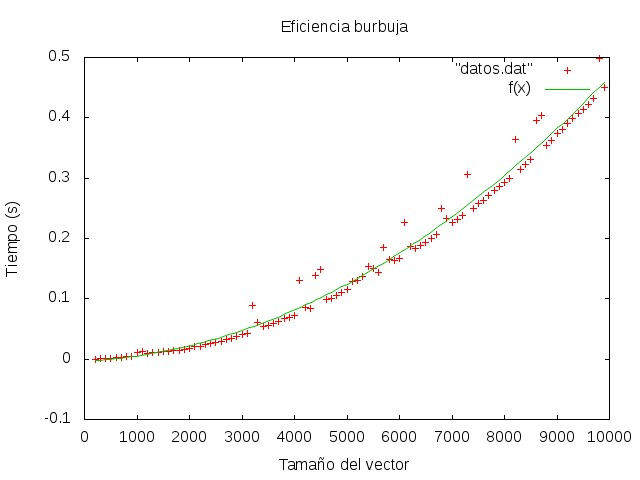
\includegraphics[scale=0.55]{../Graficas/Burbuja/burbujaO0_ruben.jpeg}
\end{center}

\subsubsection{Inserci\'on} %%%%%%%%%%%%%%%%%%%%%%%%%%%%%%%%%%%%%%%%55
$f(x) = a\cdot x^2 + b\cdot x + c \implies$
$\left\{ \begin{array}{c}
a               = 2.36229\cdot 10^{-9}      \pm 2.503\cdot 10^{-10}    (10.6\%) \\
b               = -2.27723\cdot 10^{-6}     \pm 2.606\cdot 10^{-6}    (114.5\%) \\
c               = 0.00096037       \pm 0.005712     (594.8\%)
\end{array}\right.$

\begin{center}
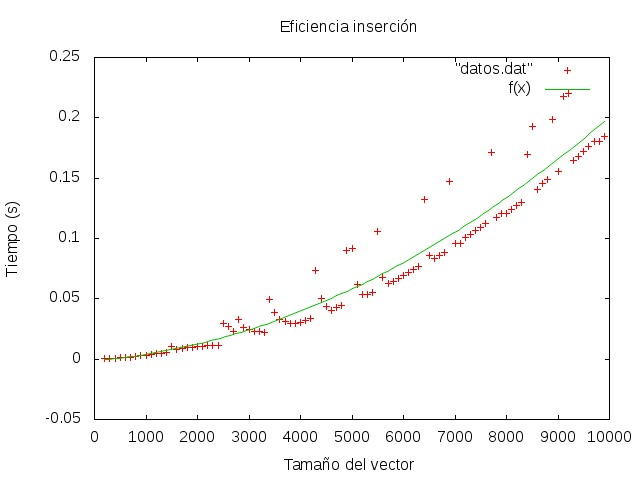
\includegraphics[scale=0.55]{../Graficas/Insercion/insercionO0_ruben.jpeg}
\end{center}

\newpage
\subsubsection{Selecci\'on}
$f(x) = a\cdot x^2 + b\cdot x + c \implies$
$ a               = 2.36327\cdot 10^{-9}      \pm 3.232\cdot 10^{-11}    (1.368\%) $
\begin{center}
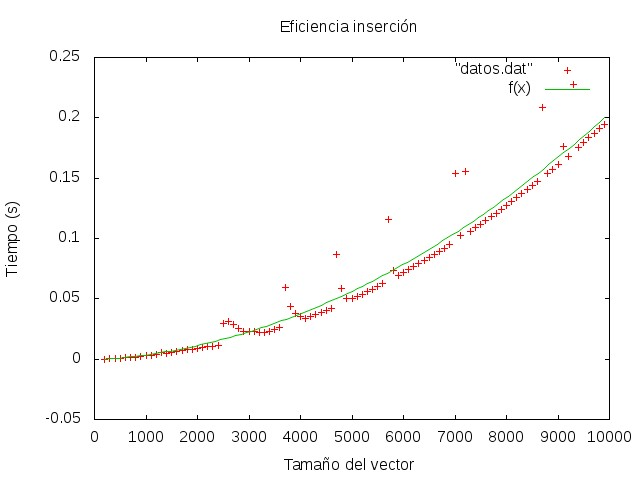
\includegraphics[scale=0.55]{../Graficas/Seleccion/seleccionO0_ruben.jpeg}
\end{center}

{\ }

\subsubsection{Mergesort}
$ f(x) = a\cdot x\cdot log_2(x) \implies$
$ a               = 3.5231\cdot 10^{-8}       \pm 1.191\cdot 10^{-9}    (3.382\%) $
\begin{center}
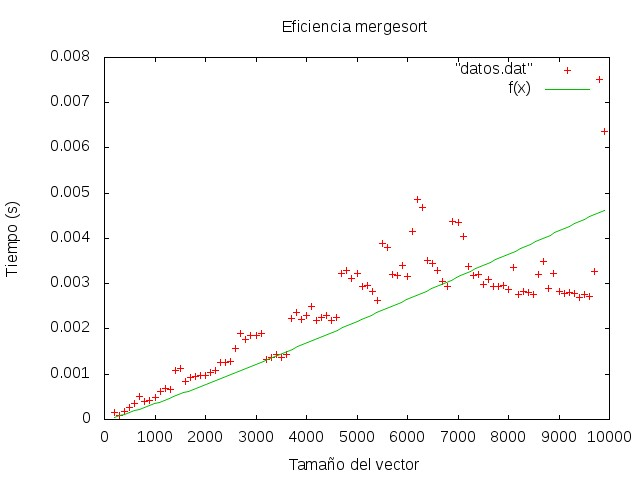
\includegraphics[scale=0.55]{../Graficas/Mergesort/mergesortO0_ruben.jpeg}
\end{center}
\newpage

\subsubsection{Quicksort}
$ f(x) = a\cdot x\cdot log_2(x) \implies$
$ a               = 2.3704\cdot 10^{-8}       \pm 5.497\cdot 10^{-10}    (2.319\%) $
\begin{center}
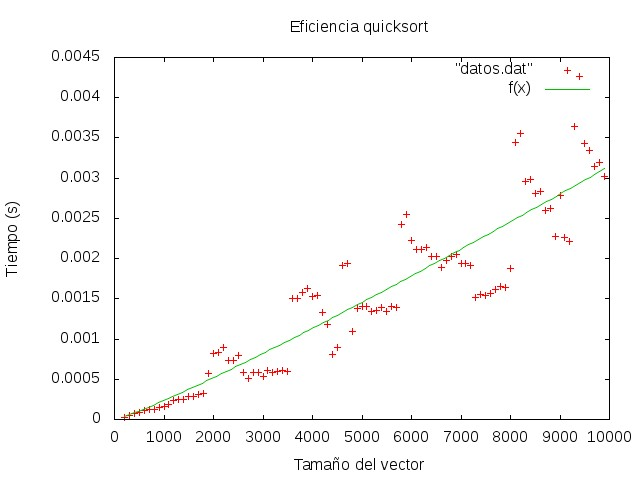
\includegraphics[scale=0.55]{../Graficas/Quicksort/quicksortO0_ruben.jpeg}
\end{center}

\subsubsection{Heapsort}
$ f(x) = a\cdot x\cdot log_2(x) \implies$
$a               = 2.49016\cdot 10^{-8}      \pm 7.983\cdot 10^{-10}    (3.206\%)$
\begin{center}
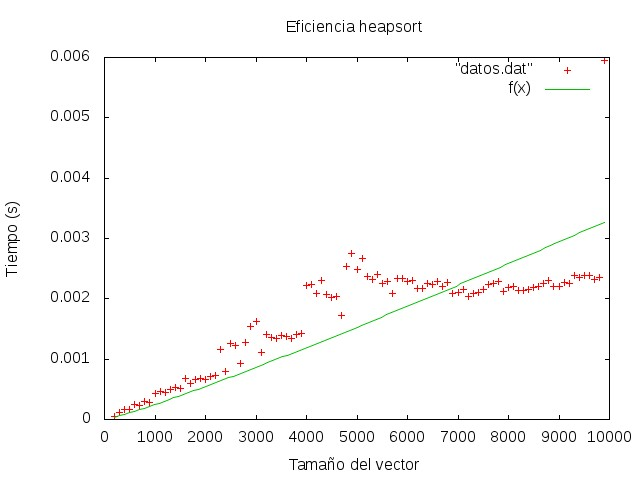
\includegraphics[scale=0.55]{../Graficas/Heapsort/heapsortO0_ruben.jpeg}
\end{center}

\subsubsection{Comparativa algoritmos de ordenaci\'ion}

En este apartado comprobamos empíricamente las diferencias de eficiencia entre diferentes algoritmos de ordenación de un vector. Se observa una diferencia notable entre los algoritmos $O(nlog_2(n))$ y los $O(n^2)$, casi no se aprecian los primeros.

También nos percatamos de la diferencia dentro de los mismos algoritmos con eficiencia $O(n^2)$, debido a la constante multiplicativa que los acompaña, inserción y selección son parecidos y burbuja tarda bastante más que los anteriores.

\begin{center}
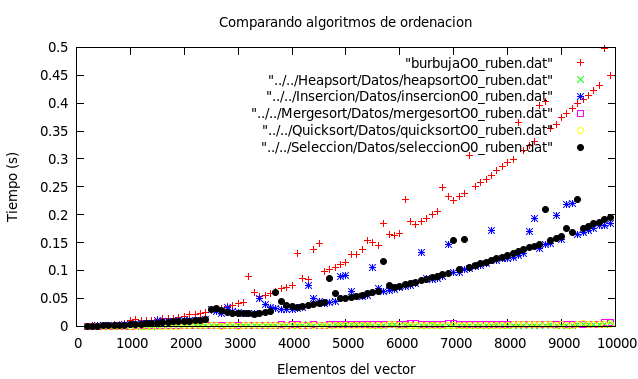
\includegraphics[scale=0.55]{../Graficas/todos.png}
\end{center}

\subsection{Fibonacci}
$ f(x) = a\cdot ((1+\sqrt(5))/2)^x \implies$
$a               = 5.59738\cdot 10^{-9}      \pm 2.093\cdot 10^{-12}    (0.0374\%)$

\begin{center}
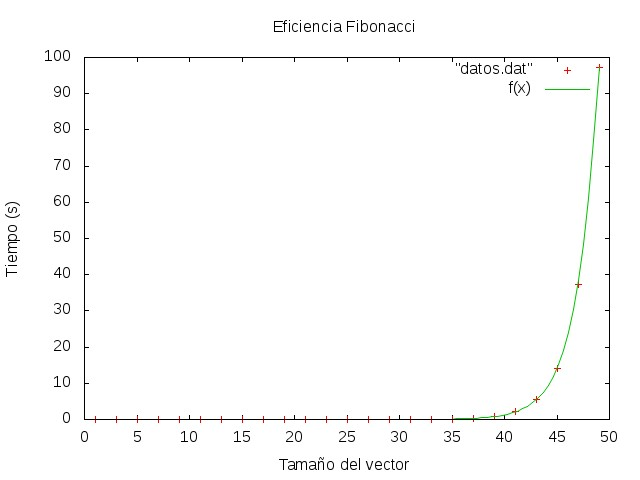
\includegraphics[scale=0.55]{../Graficas/Fibonacci/fibonacciO0_ruben.jpeg}
\end{center}
\newpage
\subsection{Hanoi}
$f(x) = a\cdot(2^x) \implies$
$a               = 1.12636\cdot 10^{-8}      \pm 1.391\cdot 10^{-11}    (0.1235\%)$
\begin{center}
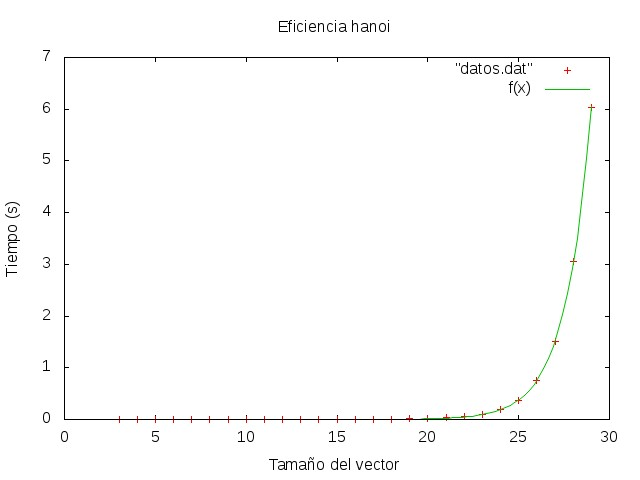
\includegraphics[scale=0.55]{../Graficas/Hanoi/hanoiO0_ruben.jpeg}
\end{center}


\subsection{Floyd}
$f(x) = a\cdot x^3 + b\cdot x^2 + c\cdot x + d \implies$
$\left\{ \begin{array}{c}
a               = 1.11725\cdot 10^{-8}      \pm 3.725\cdot 10^{-10}    (3.334\%) \\
b               = -2.27723\cdot 10^{-6}     \pm 6.692\cdot 10^{-7}    (29.39\%) \\
c               = 0.00096037       \pm 0.0003713    (38.66\%) \\
d               = -0.115743        \pm 0.06234      (53.86\%)
\end{array}\right.$

\begin{center}
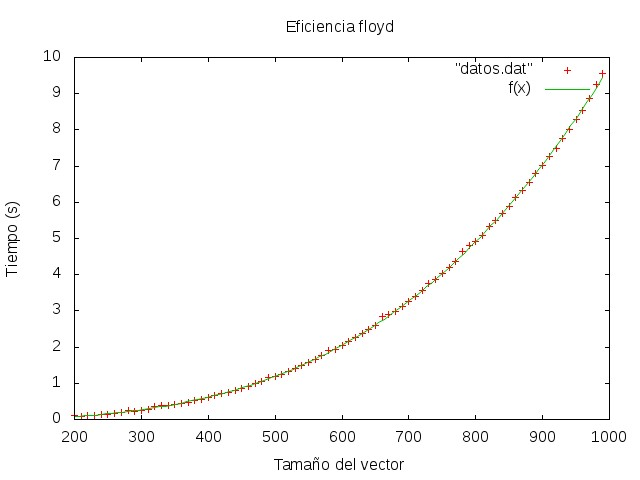
\includegraphics[scale=0.55]{../Graficas/Floyd/floydO0_ruben.jpeg}
\end{center}
\newpage

\subsection{Optimizaci\'on de algunos algoritmos}
Como podemos comprobar, por mucho que optimicemos el algoritmo de burbuja no llega a igualarse al mejor algoritmo de ordenación (en término medio), quicksort. La optimización más agresiva sin riesgo de pérdida de información es -O2 y llega a ser 10 veces más lento que quicksort sin optimización (con 10.000 elementos).

Esto es una prueba gráfica de que hay que tener en cuenta la eficiencia de los algoritmos, ya que la mejora hardware no es suficiente en caso de que tengamos restricciones de tiempo.

\begin{center}
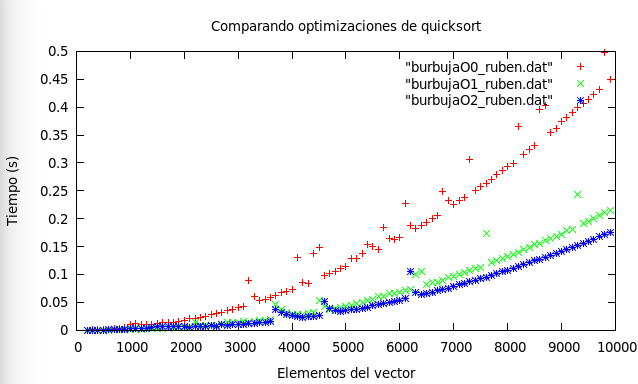
\includegraphics[scale=0.55]{../Graficas/Burbuja/burbuja_optimizacion.png}
\end{center}

Una observación curiosa es que el algoritmo Quicksort realmente es un algoritmo con eficiencia en el caso peor de $O(n^2)$, ya que si le pasamos un vector que está ordenado es cuadrático. Por otro lado Heapsort es un $O(nlog_2(n))$ puro, pero en término medio es peor que Quicksort, ya que los datos que se suelen pasar a estos algoritmos no están ordenados.

\begin{center}
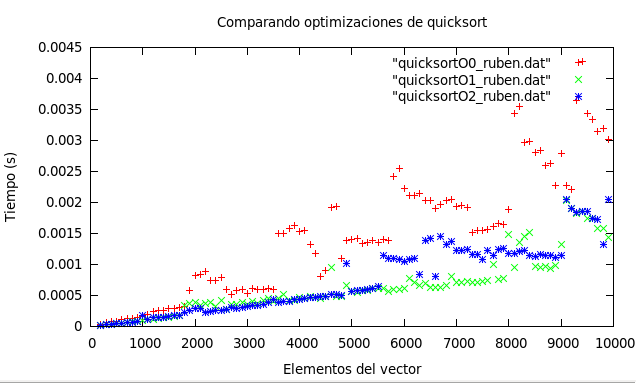
\includegraphics[scale=0.55]{../Graficas/Quicksort/quicksort_optimizacion.png}
\end{center}

{\ }

Después de comparar dichos algoritmos de ordenación optimizaremos el algoritmo floyd, tipo de algoritmo con programación dinámica para encontrar el camino mínimo en grafos ponderados.

\begin{center}
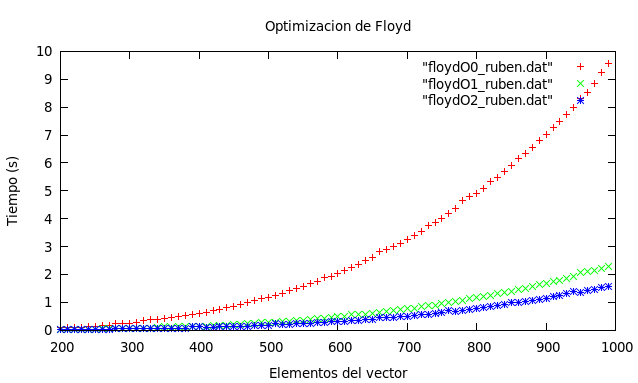
\includegraphics[scale=0.55]{../Graficas/Floyd/floyd_optimizacion.png}
\end{center}

\subsection{Diferentes ordenadores}
Si ejecutamos el mismo programa en diferentes ordenadores este será el resultado.

\begin{center}
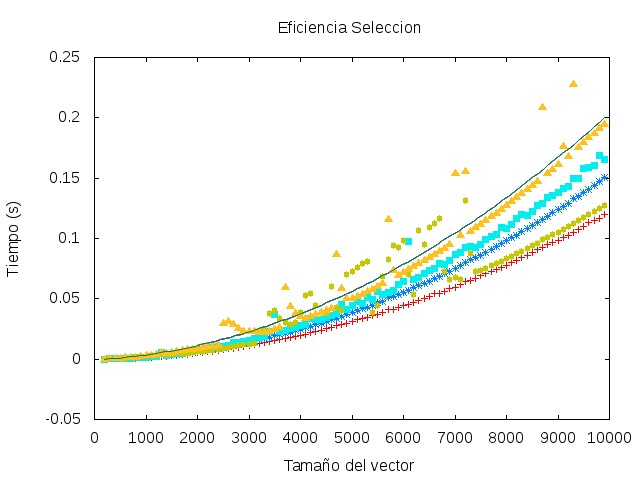
\includegraphics[scale=0.55]{../Graficas/Seleccion/total_Seleccion.jpeg}
\end{center}	

\begin{center}
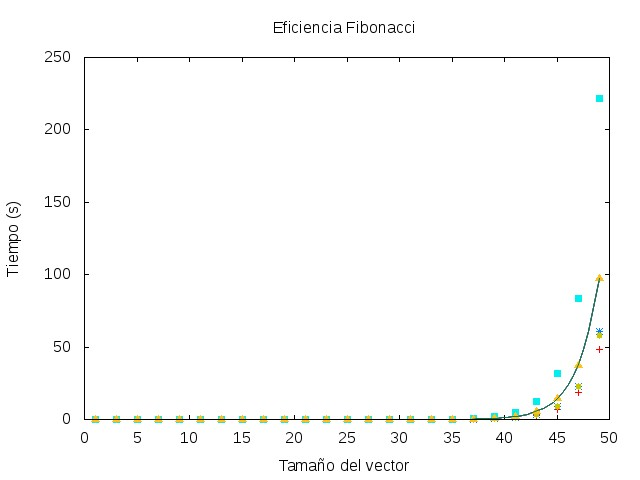
\includegraphics[scale=0.55]{../Graficas/Fibonacci/total_Fibonacci.jpeg}
\end{center}

\begin{center}
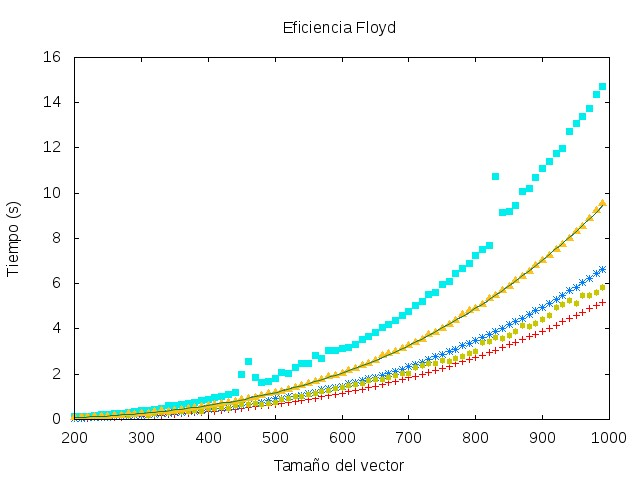
\includegraphics[scale=0.55]{../Graficas/Floyd/total_Floyd.jpeg}
\end{center}

\section{Ordenador usado para la ejecuci\'on}
HP Pavilion g series (Pavilion g6)

Sistema operativo: ubuntu 14.04 LTS

Memoria: 3.8 GiB (4Gb)

Procesador: Inter Core i3-2330M CPU @ 2.20GHz x 4

Gráficos: Intel Sandybridge Mobile

Tipo de SO: 64 bits

Disco: 487.9 GB

\newpage
%%%%%%%%%%%%%%%%%%%%%%%%%%%%%%%%%%%%%%%%%%%%%%%%%%%%%%%%%%%%%%%%%%%%%%%%%%%%%%%%%%

% % % % % % % % % % % % % % % % % % % % % % % % % % % % % % % % %
%					 Bibliografía
% % % % % % % % % % % % % % % % % % % % % % % % % % % % % % % % %
\section{Bibliografia}
\url{http://www.rinconmatematico.com/instructivolatex/formulas.htm}

\url{http://osl.ugr.es/CTAN/macros/latex/contrib/beamer/doc/beameruserguide.pdf}

\url{https://github.com/dgiim/beamer}

\url{http://www.tablesgenerator.com/}

\url{https://es.wikipedia.org/wiki/Algoritmo_de_Floyd-Warshall}

\end{document}
